\thispagestyle{plain}

\noindent In the first part of this project a function called Franke function
 was used as the data analysed. The Franke function is given by the following 
 equation:
\begin{align*}
    f(x,y) &= \frac{3}{4} \, exp\left(- \frac{(9x-2)^2}{4} - \frac{(9y-2)^2}{4}\right) \\
    &+ \frac{3}{4}\, exp\left( - \frac{(9x +1)^2}{49} - \frac{(9y+1)}{10}\right) \\
    &+ \frac{1}{2}\, exp\left( -\frac{(9x-7)^2}{4} - \frac{(9y-3)^2}{4}\right) \\
    &- \frac{1}{5} exp \left( - (9x -4)^2 - (9y-7)^2\right)
\end{align*}
%A graphic representation is shown in figure \eqref{Franke function}
\begin{figure}[H]
	\centering
	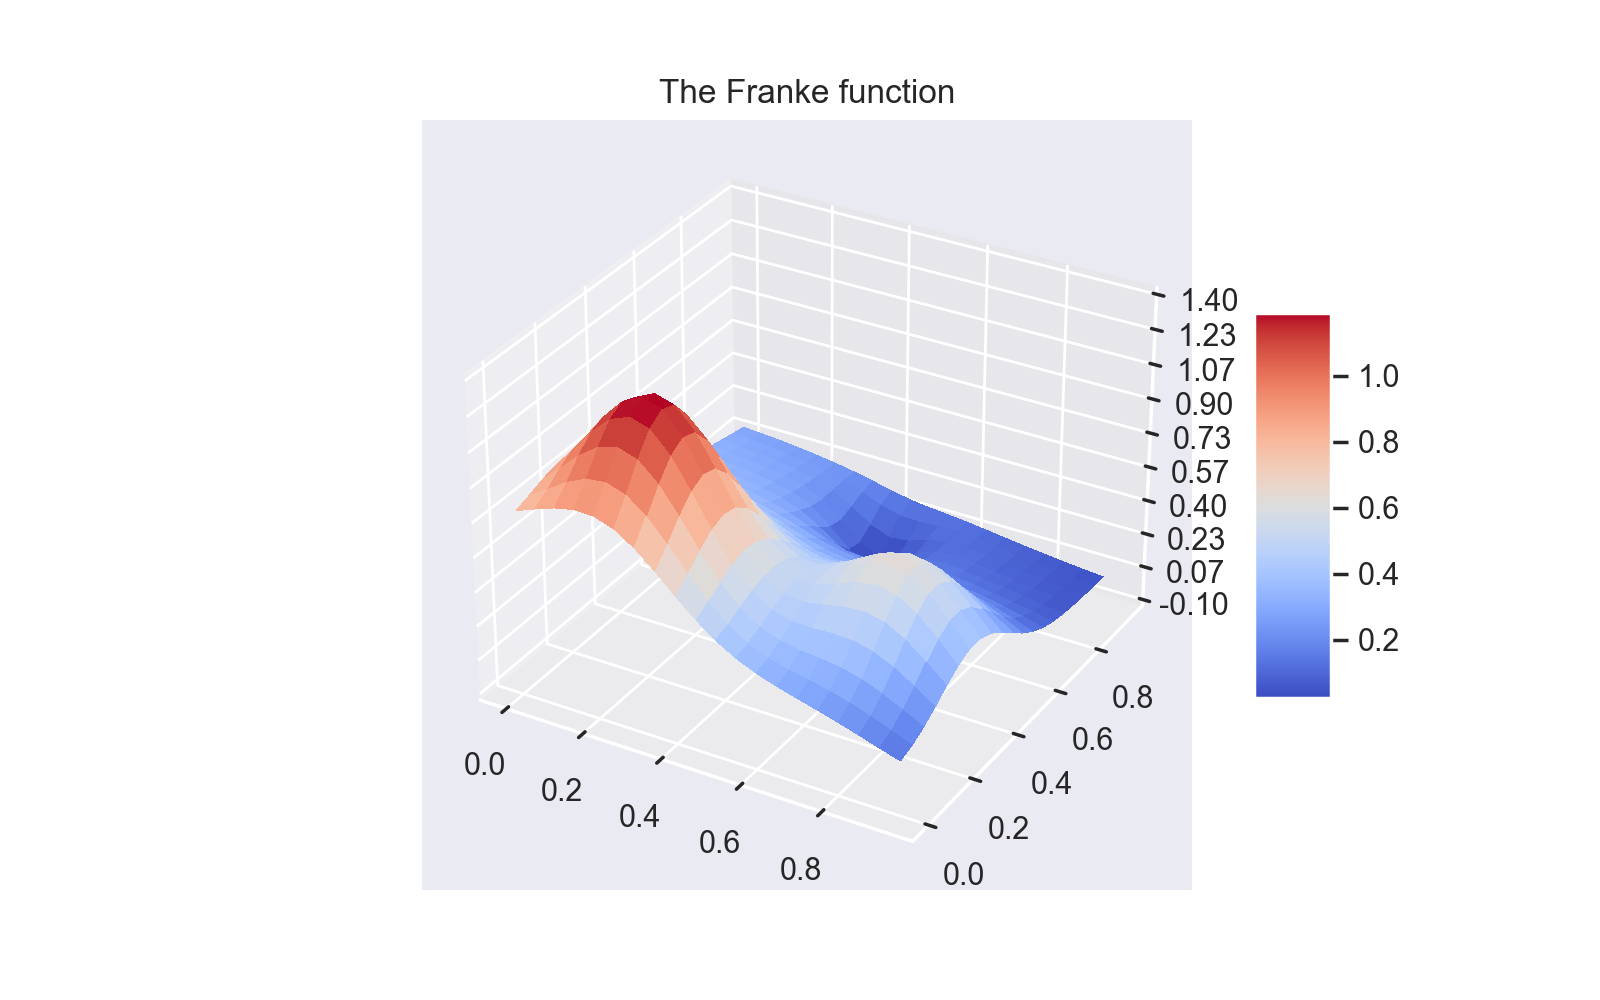
\includegraphics[width=0.5\textwidth]{Figure_1.png}
	\caption{\centering A plot of the Franke function }
	\label{Franke function}
\end{figure}
\noindent This function was fitted with the OLS method, 
and polynomials with varying degrees was used to create the design matrix.
Since the design matrix in this case was noninvertible, singular value 
decomposition was used to create the $\beta$-values needed to create a model
of the dataset. The mean square error and the R2 score was calculated 
for both the testing and training datasets. The result of this analyses is 
shown if figures \eqref{MSE and R2 OLS}, \eqref{MSE and R2 OLS noise} and ...

\noindent Next Ridge and LASSO regression was used on the Franke function,
to see if these methods have a better fit than what was obtained with OLS.
Diffrent values for $\lambda$ was used to obtain the best fit as possible for each
polynomial degree.

\subsection{Cross Validation Methodology}

In the pursuit of assessing the robustness and reliability of Ridge regression models, we employed cross-validation, specifically scrutinizing the impact of varying regularization parameters, denoted as \(\lambda\). The function \texttt{k\_fold}, was developed to execute the k-fold cross-validation technique, accepting the dataset and an integer \(k\) as arguments, and subsequently partitioning the data into \(k\) randomized subsets (folds). It returns \(k\) pairs of training and test indices, each representing a distinct division of the data, enabling model evaluation across varied data scenarios.

For each \(\lambda\) value in a logarithmically spaced array of \(\lambda\) values, denoted \texttt{lambdas}, the Ridge regression model was trained and validated \(k\) times - once per fold. Specifically, for every tuple \((\text{train\_indices}, \text{test\_indices})\) produced by \texttt{k\_fold(data, k)}, the data was divided into training and test sets \((x_{\text{train}}, y_{\text{train}}, x_{\text{test}}, y_{\text{test}})\).
Subsequently, the \texttt{design\_matrix} function generated polynomial feature matrices \(X_{\text{train}}\) and \(X_{\text{test}}\) from the \(x\) and \(y\) values, using a specified polynomial degree. 

The Ridge model, instantiated with the current \(\lambda\), was then fitted with \(X_{\text{train}}\) and \(y_{\text{train}}\), and predictions \(y_{\text{pred}}\) were made using \(X_{\text{test}}\). The Mean Squared Error (MSE) between the predictions and actual test values \(y_{\text{test}}\) was computed and stored in a scores array.
The MSE values were averaged per \(\lambda\), providing an unbiased performance metric, and facilitating the analysis and visualization of how distinct regularization parameters influenced model performance.
